\documentclass[aspectratio = 43]{beamer}
\usetheme{Madrid}
\usepackage{pdfpages}
\usepackage{hyperref}
\title{Logic}
\begin{document}

\maketitle
\begin{frame}{TOC}
\tableofcontents[sections=1-8]
\end{frame}
\begin{frame}{TOC}
\tableofcontents[sections=9-16]
\end{frame}
\begin{frame}{TOC}
\tableofcontents[sections=17-24]
\end{frame}
\begin{frame}{TOC}
\tableofcontents[sections=25-32]
\end{frame}
\begin{frame}{TOC}
\tableofcontents[sections=33-34]
\end{frame}
\section{Lecture 00 Motivation.pdf}
\begin{frame}{Lecture 00 Motivation.pdf}
\end{frame}
\includepdf[pages=-]{../Lecture_00_Motivation.pdf}
\section{Lecture 01 Natural Deduction 1.pdf}
\begin{frame}{Lecture 01 Natural Deduction 1.pdf}
\end{frame}
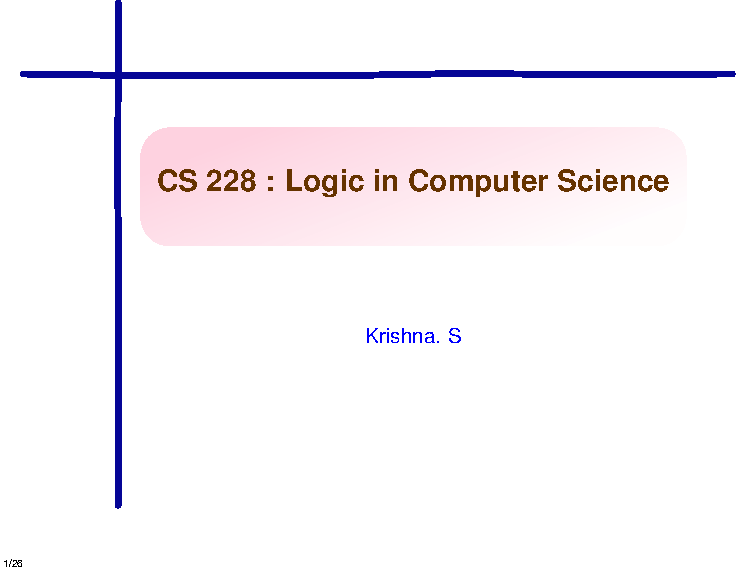
\includepdf[pages=-]{../Lecture_01_Natural_Deduction_1.pdf}
\section{Lecture 02 Natural Deduction 2.pdf}
\begin{frame}{Lecture 02 Natural Deduction 2.pdf}
\end{frame}
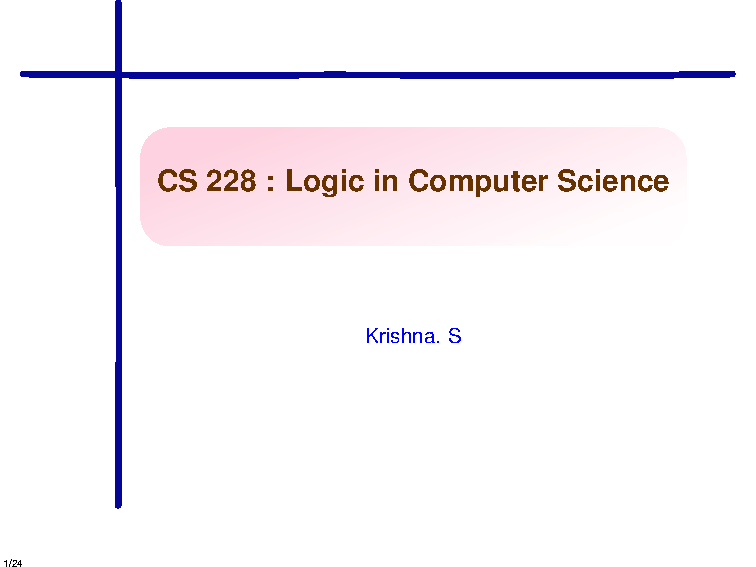
\includepdf[pages=-]{../Lecture_02_Natural_Deduction_2.pdf}
\section{Lecture 03 Soundness and Completeness Of PL.pdf}
\begin{frame}{Lecture 03 Soundness and Completeness Of PL.pdf}
\end{frame}
\includepdf[pages=-]{../Lecture_03_Soundness_and_Completeness_Of_PL.pdf}
\section{Lecture 04 Normal Forms and Horn Clauses.pdf}
\begin{frame}{Lecture 04 Normal Forms and Horn Clauses.pdf}
\end{frame}
\includepdf[pages=-]{../Lecture_04_Normal_Forms_and_Horn_Clauses.pdf}
\section{Lecture 05 Resolution 1.pdf}
\begin{frame}{Lecture 05 Resolution 1.pdf}
\end{frame}
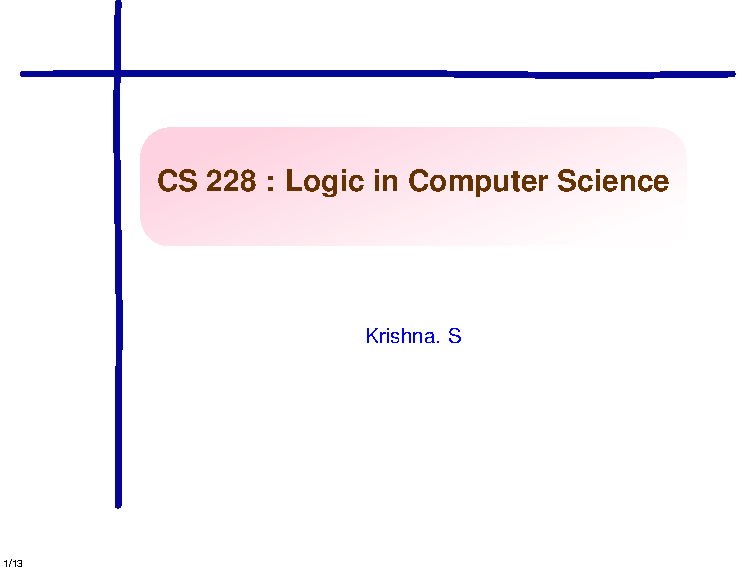
\includepdf[pages=-]{../Lecture_05_Resolution_1.pdf}
\section{Lecture 06 Resolution 2.pdf}
\begin{frame}{Lecture 06 Resolution 2.pdf}
\end{frame}
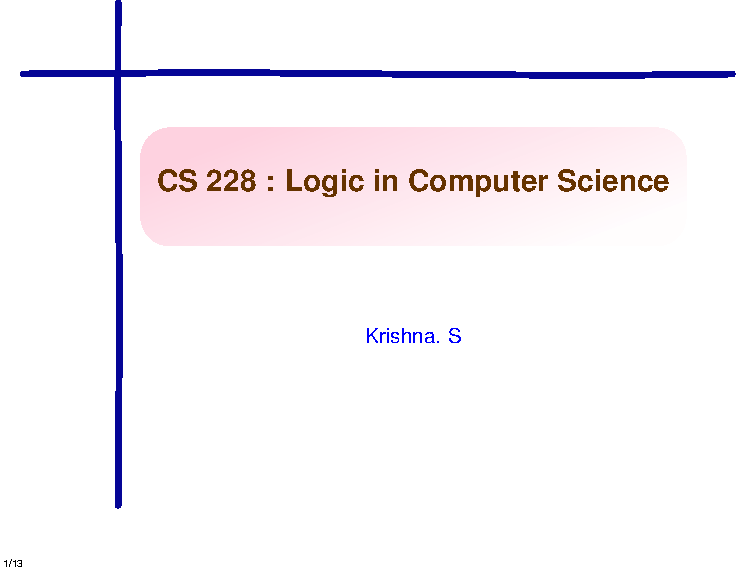
\includepdf[pages=-]{../Lecture_06_Resolution_2.pdf}
\section{Lecture 07 Recap.pdf}
\begin{frame}{Lecture 07 Recap.pdf}
\end{frame}
\includepdf[pages=-]{../Lecture_07_Recap.pdf}
\section{Lecture 08 CNF to DNF.pdf}
\begin{frame}{Lecture 08 CNF to DNF.pdf}
\end{frame}
\includepdf[pages=-]{../Lecture_08_CNF_to_DNF.pdf}
\section{Lecture 09 DPLL.pdf}
\begin{frame}{Lecture 09 DPLL.pdf}
\end{frame}
\includepdf[pages=-]{../Lecture_09_DPLL.pdf}
\section{Lecture 10 FOL Syntax.pdf}
\begin{frame}{Lecture 10 FOL Syntax.pdf}
\end{frame}
\includepdf[pages=-]{../Lecture_10_FOL_Syntax.pdf}
\section{Lecture 11 FOL Semantics.pdf}
\begin{frame}{Lecture 11 FOL Semantics.pdf}
\end{frame}
\includepdf[pages=-]{../Lecture_11_FOL_Semantics.pdf}
\section{Lecture 12 FOL SAT.pdf}
\begin{frame}{Lecture 12 FOL SAT.pdf}
\end{frame}
\includepdf[pages=-]{../Lecture_12_FOL_SAT.pdf}
\section{Lecture 13 FOL SAT Translation.pdf}
\begin{frame}{Lecture 13 FOL SAT Translation.pdf}
\end{frame}
\includepdf[pages=-]{../Lecture_13_FOL_SAT_Translation.pdf}
\section{Lecture 14 FOL RPF Skolemisation.pdf}
\begin{frame}{Lecture 14 FOL RPF Skolemisation.pdf}
\end{frame}
\includepdf[pages=-]{../Lecture_14_FOL_RPF_Skolemisation.pdf}
\section{Lecture 15 FOL Words.pdf}
\begin{frame}{Lecture 15 FOL Words.pdf}
\end{frame}
\includepdf[pages=-]{../Lecture_15_FOL_Words.pdf}
\section{Lecture 16 FOL FSM 01.pdf}
\begin{frame}{Lecture 16 FOL FSM 01.pdf}
\end{frame}
\includepdf[pages=-]{../Lecture_16_FOL_FSM_01.pdf}
\section{Lecture 17 FOL FSM 02.pdf}
\begin{frame}{Lecture 17 FOL FSM 02.pdf}
\end{frame}
\includepdf[pages=-]{../Lecture_17_FOL_FSM_02.pdf}
\section{Lecture 18 FOL NFA.pdf}
\begin{frame}{Lecture 18 FOL NFA.pdf}
\end{frame}
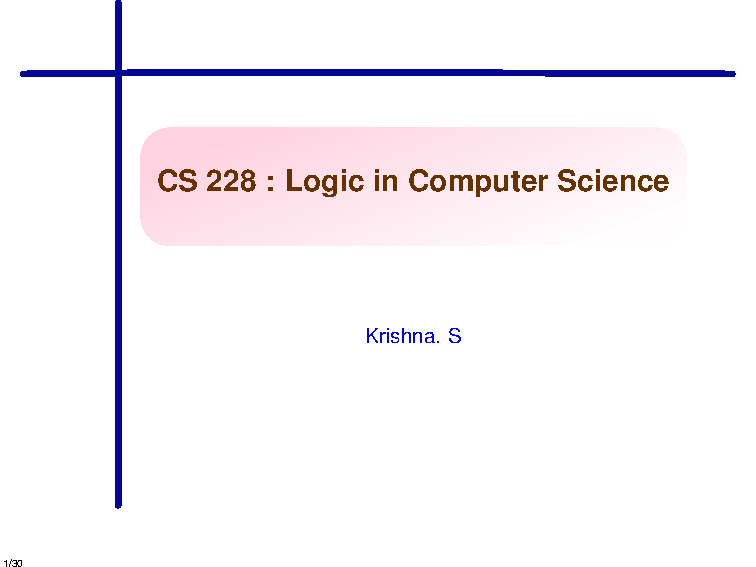
\includepdf[pages=-]{../Lecture_18_FOL_NFA.pdf}
\section{Lecture 19 FOL NFA to DFA 1.pdf}
\begin{frame}{Lecture 19 FOL NFA to DFA 1.pdf}
\end{frame}
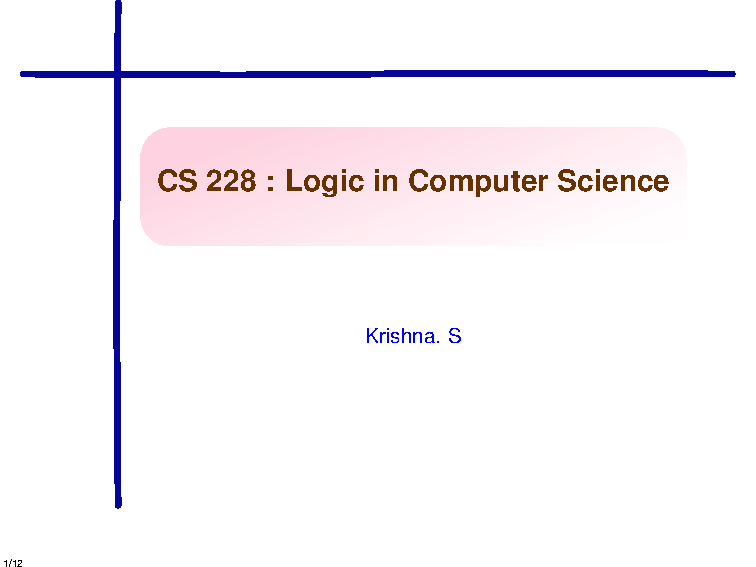
\includepdf[pages=-]{../Lecture_19_FOL_NFA_to_DFA_1.pdf}
\section{Lecture 20 FOL NFA to DFA 2.pdf}
\begin{frame}{Lecture 20 FOL NFA to DFA 2.pdf}
\end{frame}
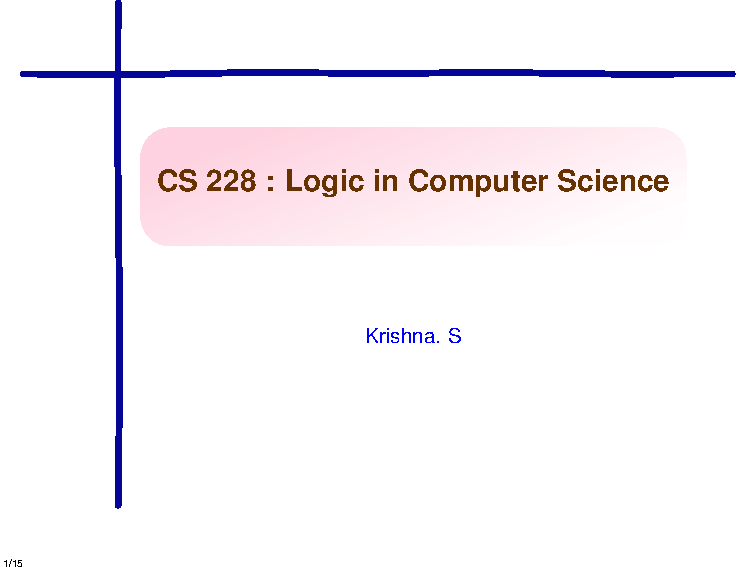
\includepdf[pages=-]{../Lecture_20_FOL_NFA_to_DFA_2.pdf}
\section{Lecture 21 FOL NFA to DFA 3.pdf}
\begin{frame}{Lecture 21 FOL NFA to DFA 3.pdf}
\end{frame}
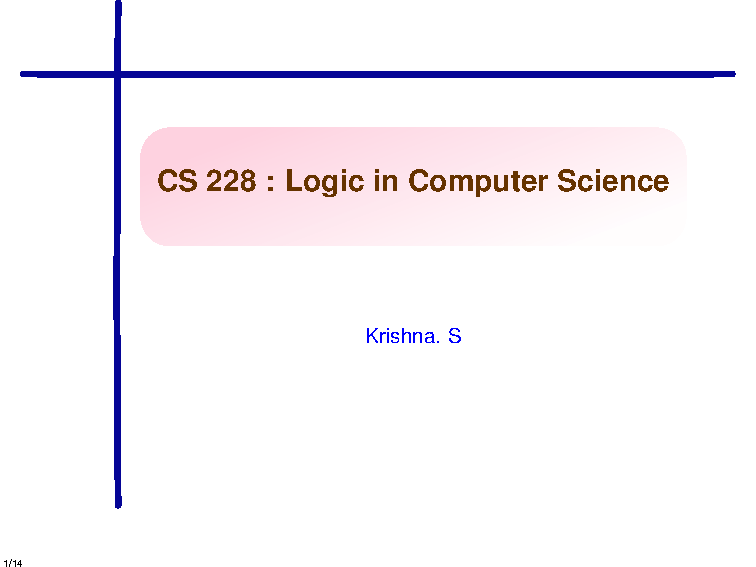
\includepdf[pages=-]{../Lecture_21_FOL_NFA_to_DFA_3.pdf}
\section{Lecture 22 MSO.pdf}
\begin{frame}{Lecture 22 MSO.pdf}
\end{frame}
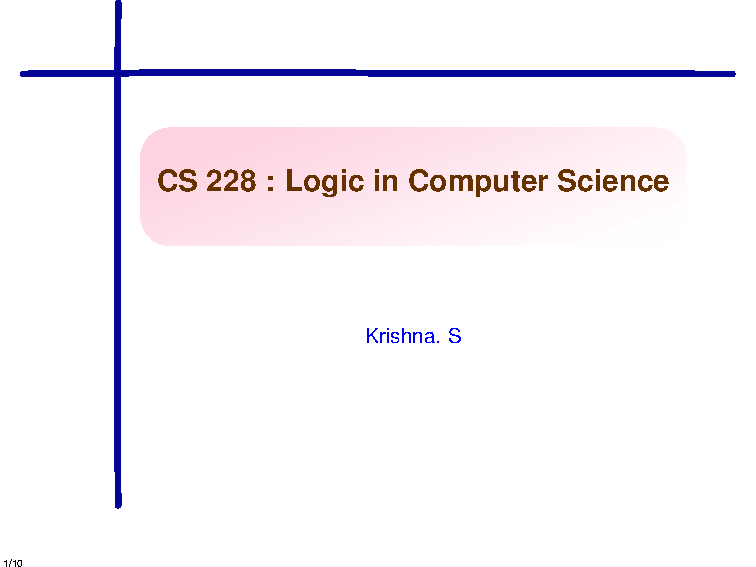
\includepdf[pages=-]{../Lecture_22_MSO.pdf}
\section{Lecture 23 MSO Regular Languages.pdf}
\begin{frame}{Lecture 23 MSO Regular Languages.pdf}
\end{frame}
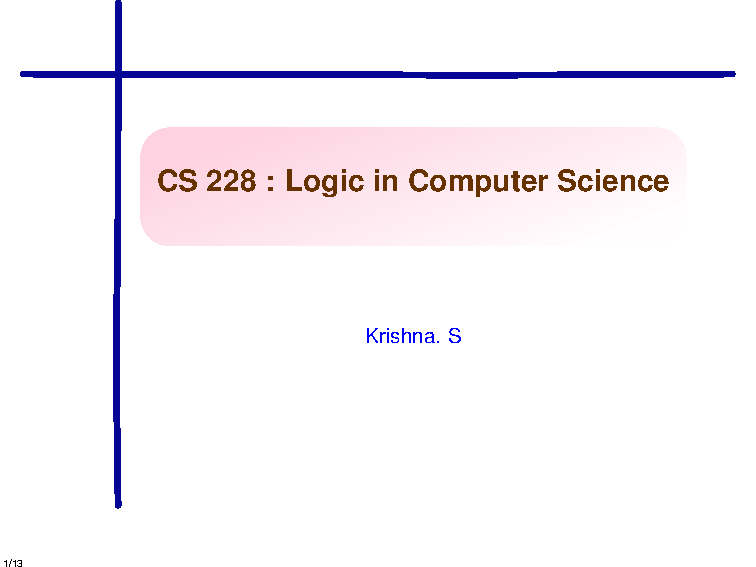
\includepdf[pages=-]{../Lecture_23_MSO_Regular_Languages.pdf}
\section{Lecture 24 Herbrand Theory.pdf}
\begin{frame}{Lecture 24 Herbrand Theory.pdf}
\end{frame}
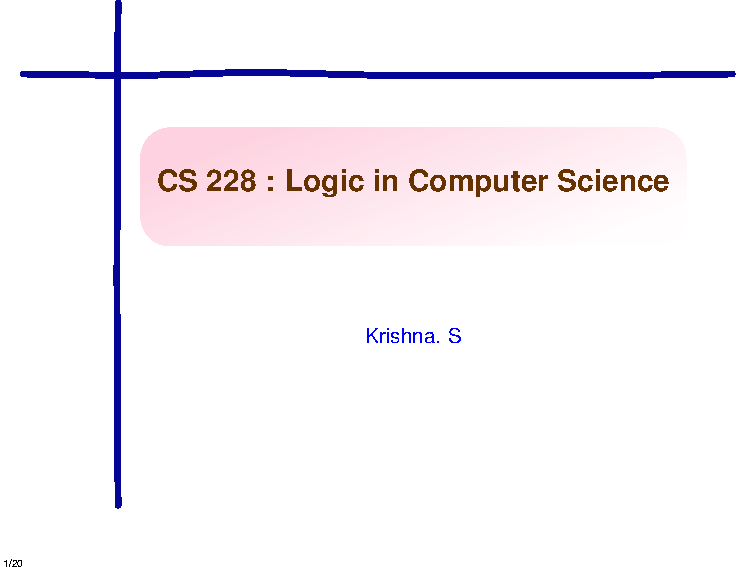
\includepdf[pages=-]{../Lecture_24_Herbrand_Theory.pdf}
\section{Lecture 25 Herbrand Theorem.pdf}
\begin{frame}{Lecture 25 Herbrand Theorem.pdf}
\end{frame}
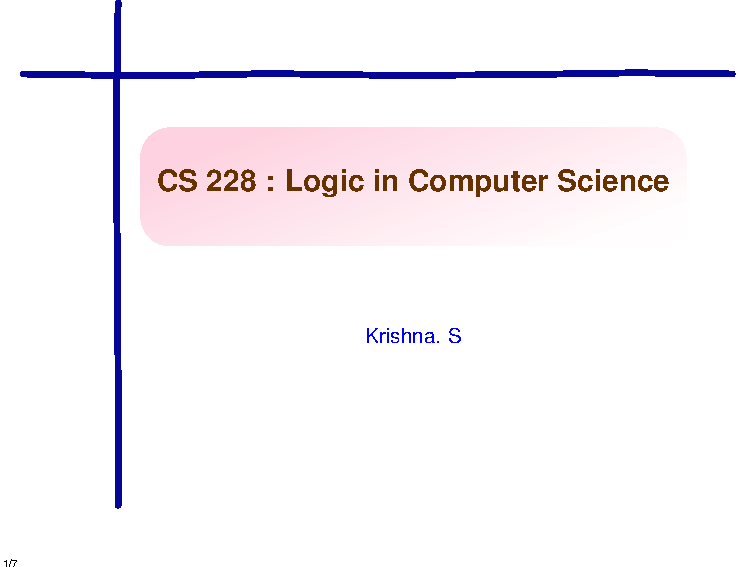
\includepdf[pages=-]{../Lecture_25_Herbrand_Theorem.pdf}
\section{Lecture 26 Herbrand Method.pdf}
\begin{frame}{Lecture 26 Herbrand Method.pdf}
\end{frame}
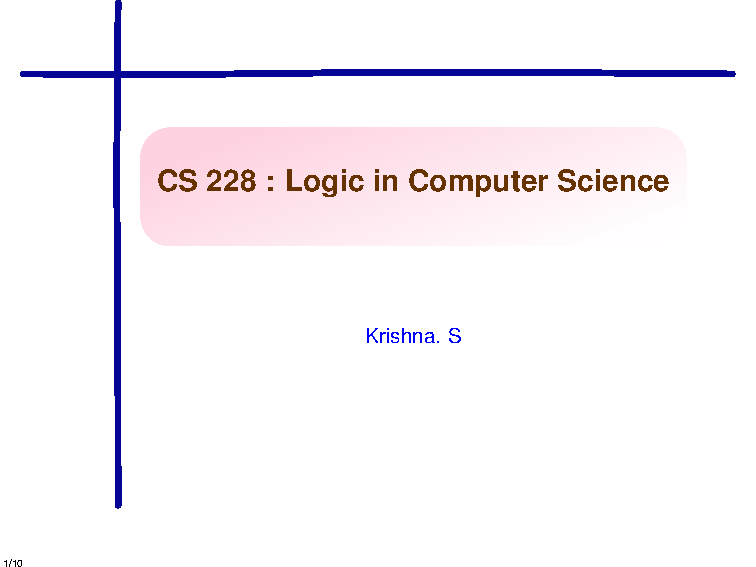
\includepdf[pages=-]{../Lecture_26_Herbrand_Method.pdf}
\section{Lecture 27-29 LTL Transitions DBA and NBA.pdf}
\begin{frame}{Lecture 27-29 LTL Transitions DBA and NBA.pdf}
\end{frame}
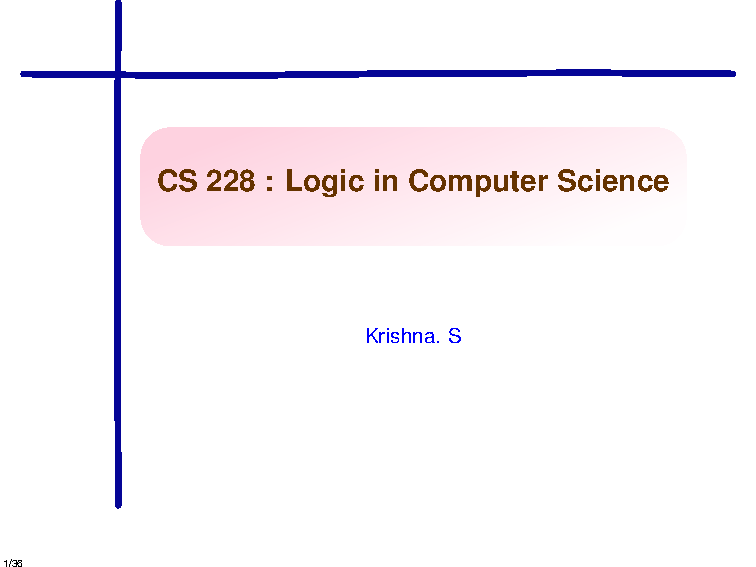
\includepdf[pages=-]{../Lecture_27-29_LTL_Transitions_DBA_and_NBA.pdf}
\section{Lecture 27 Model Checking LTL.pdf}
\begin{frame}{Lecture 27 Model Checking LTL.pdf}
\end{frame}
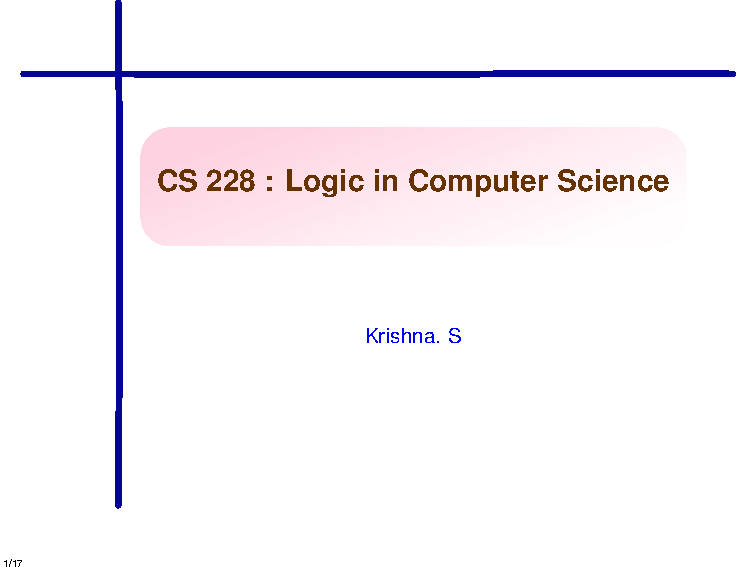
\includepdf[pages=-]{../Lecture_27_Model_Checking_LTL.pdf}
\section{Lecture 28-29 LTL.pdf}
\begin{frame}{Lecture 28-29 LTL.pdf}
\end{frame}
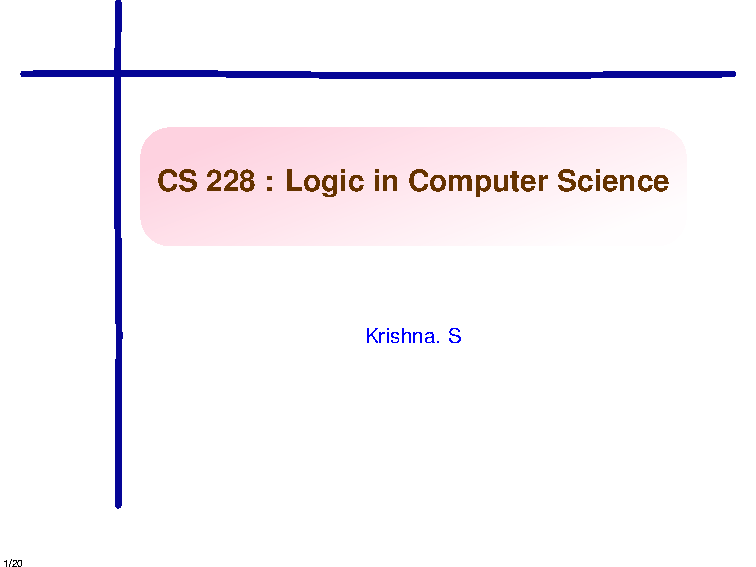
\includepdf[pages=-]{../Lecture_28-29_LTL.pdf}
\section{Lecture 30.pdf}
\begin{frame}{Lecture 30.pdf}
\end{frame}
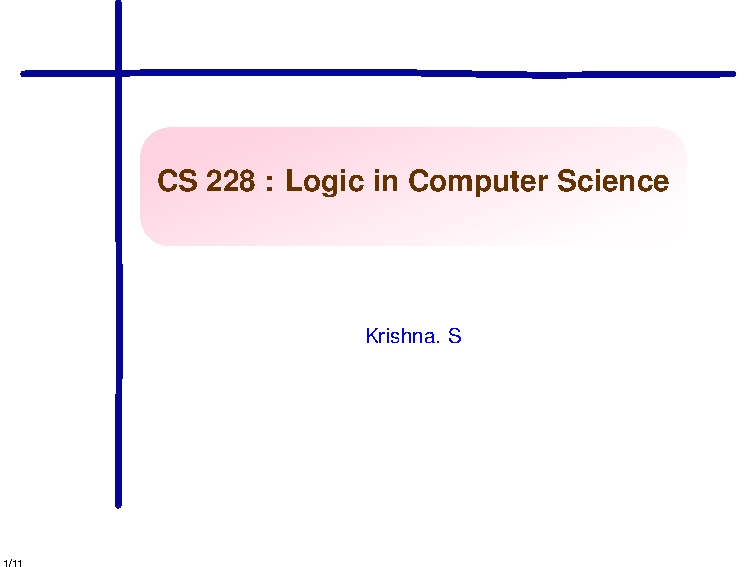
\includepdf[pages=-]{../Lecture_30.pdf}
\section{Lecture 31.pdf}
\begin{frame}{Lecture 31.pdf}
\end{frame}
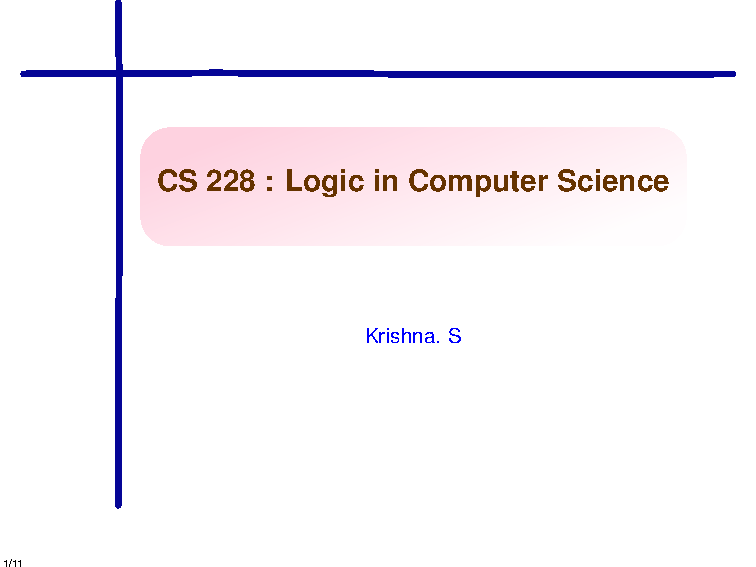
\includepdf[pages=-]{../Lecture_31.pdf}
\section{Lecture 32-34.pdf}
\begin{frame}{Lecture 32-34.pdf}
\end{frame}
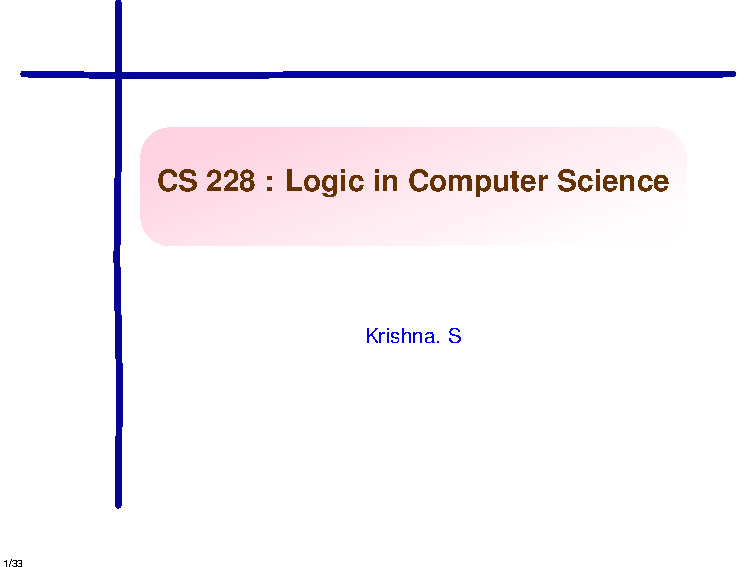
\includepdf[pages=-]{../Lecture_32-34.pdf}
\section{Lecture 36.pdf}
\begin{frame}{Lecture 36.pdf}
\end{frame}
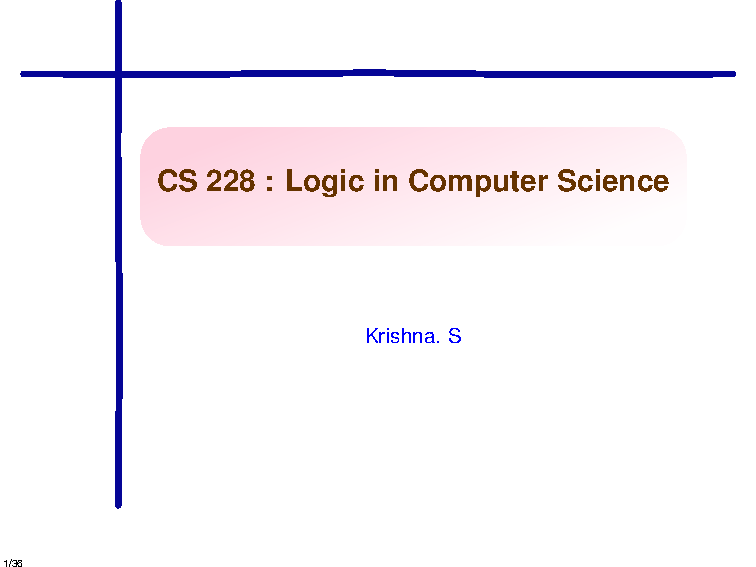
\includepdf[pages=-]{../Lecture_36.pdf}
\newpage

\end{document}
